%=============================================================================
%  Half-Life Estimation — Mathematical Notes & Documentation
%  Study Notes + Technical Reference | Dark Wing Project
%=============================================================================
\documentclass[10pt,a4paper,twocolumn]{article}

%--- Geometry ----------------------------------------------------------------
\usepackage[a4paper,top=1.8cm,bottom=1.8cm,left=1.5cm,right=1.5cm,
            columnsep=0.7cm]{geometry}

%--- Math --------------------------------------------------------------------
\usepackage{amsmath,amssymb,amsthm,mathtools}

%--- Typography --------------------------------------------------------------
\usepackage[T1]{fontenc}
\usepackage{lmodern}
\usepackage{microtype}
\usepackage{parskip}
\setlength{\parskip}{2pt}

%--- Colours -----------------------------------------------------------------
\usepackage{xcolor}
\definecolor{codebg}{RGB}{245,247,250}
\definecolor{codeframe}{RGB}{180,195,220}
\definecolor{keyword}{RGB}{0,80,180}
\definecolor{comment}{RGB}{80,115,80}
\definecolor{string}{RGB}{160,40,20}
\definecolor{mathbluebg}{RGB}{230,240,255}
\definecolor{mathblue}{RGB}{10,60,160}
\definecolor{accent}{RGB}{25,95,195}
\definecolor{greenbg}{RGB}{230,250,232}
\definecolor{greenframe}{RGB}{50,155,70}
\definecolor{yellowbg}{RGB}{255,252,230}
\definecolor{yellowframe}{RGB}{180,150,0}
\definecolor{notebg}{RGB}{248,245,255}
\definecolor{noteframe}{RGB}{120,80,180}

%--- Code listings -----------------------------------------------------------
\usepackage{listings}
\lstdefinestyle{python}{
  language=Python,
  backgroundcolor=\color{codebg},
  frame=single,rulecolor=\color{codeframe},
  basicstyle=\ttfamily\fontsize{6.5}{8}\selectfont,
  keywordstyle=\bfseries\color{keyword},
  commentstyle=\itshape\color{comment},
  stringstyle=\color{string},
  numbers=left,numberstyle=\tiny\color{gray!70},
  numbersep=4pt,breaklines=true,tabsize=2,
  showstringspaces=false,aboveskip=3pt,belowskip=3pt,
  xleftmargin=12pt,
}
\lstdefinestyle{pythonplain}{
  language=Python,
  backgroundcolor=\color{codebg},
  frame=single,rulecolor=\color{codeframe},
  basicstyle=\ttfamily\fontsize{6.5}{8}\selectfont,
  keywordstyle=\bfseries\color{keyword},
  commentstyle=\itshape\color{comment},
  stringstyle=\color{string},
  numbers=none,breaklines=true,tabsize=2,
  showstringspaces=false,aboveskip=3pt,belowskip=3pt,
  xleftmargin=4pt,
}

%--- TikZ --------------------------------------------------------------------
\usepackage{tikz}
\usetikzlibrary{shapes.geometric,arrows.meta,positioning,calc,
                backgrounds,decorations.pathreplacing,fit}
\raggedbottom

\tikzset{
  fc_start/.style={rectangle,rounded corners=5pt,
    draw=accent,fill=accent!18,
    text width=4.4cm,align=center,
    font=\footnotesize\bfseries,
    inner sep=4pt,minimum height=0.6cm},
  fc_proc/.style={rectangle,
    draw=black!55,fill=white,
    text width=4.4cm,align=center,
    font=\footnotesize,
    inner sep=3pt,minimum height=0.58cm},
  fc_dec/.style={diamond,aspect=2.5,
    draw=accent,fill=accent!9,
    text width=2.9cm,align=center,
    font=\fontsize{6.2}{7.2}\selectfont,
    inner sep=1pt},
  fc_out/.style={rectangle,rounded corners=3pt,
    draw=greenframe,fill=greenbg,
    text width=4.4cm,align=center,
    font=\footnotesize,
    inner sep=3pt,minimum height=0.58cm},
  fc_side/.style={rectangle,
    draw=black!45,fill=yellow!10,
    text width=2.0cm,align=center,
    font=\fontsize{6.2}{7.2}\selectfont,
    inner sep=2pt,minimum height=0.52cm},
  arr/.style={-Stealth,semithick,draw=black!65},
}

%--- Boxes -------------------------------------------------------------------
\usepackage[most]{tcolorbox}
\tcbset{
  mathbox/.style={colback=mathbluebg,colframe=mathblue,
    fonttitle=\bfseries\small,title=#1,
    boxrule=0.5pt,top=3pt,bottom=3pt,left=4pt,right=4pt,
    before skip=4pt,after skip=4pt},
  exbox/.style={colback=yellowbg,colframe=yellowframe,
    fonttitle=\bfseries\small,title=#1,
    boxrule=0.5pt,top=3pt,bottom=3pt,left=4pt,right=4pt,
    before skip=4pt,after skip=4pt},
  resultbox/.style={colback=greenbg,colframe=greenframe,
    fonttitle=\bfseries\small,title=#1,
    boxrule=0.5pt,top=3pt,bottom=3pt,left=4pt,right=4pt,
    before skip=4pt,after skip=4pt},
  codebox/.style={colback=codebg,colframe=codeframe,
    fonttitle=\bfseries\small\color{accent},title=#1,
    boxrule=0.5pt,top=2pt,bottom=2pt,left=2pt,right=2pt,
    before skip=4pt,after skip=4pt},
  notebox/.style={colback=notebg,colframe=noteframe,
    fonttitle=\bfseries\small,title=#1,
    boxrule=0.5pt,top=3pt,bottom=3pt,left=4pt,right=4pt,
    before skip=4pt,after skip=4pt},
}

%--- Tables ------------------------------------------------------------------
\usepackage{booktabs,array,multirow}

%--- Header / Footer ---------------------------------------------------------
\usepackage{fancyhdr}
\usepackage[hidelinks]{hyperref}
\pagestyle{fancy}\fancyhf{}
\fancyhead[L]{\footnotesize\textbf{Half-Life Estimation --- Study Notes}}
\fancyhead[R]{\footnotesize Project Dark-Wing}
\fancyfoot[C]{\footnotesize\thepage}
\renewcommand{\headrulewidth}{0.4pt}

%--- Floats / Captions -------------------------------------------------------
\usepackage{float,caption,graphicx}
\captionsetup{font=scriptsize,labelfont=bf,skip=3pt}

%--- Section formatting ------------------------------------------------------
\usepackage{titlesec}
\titlespacing*{\section}{0pt}{7pt}{3pt}
\titlespacing*{\subsection}{0pt}{5pt}{2pt}
\titlespacing*{\subsubsection}{0pt}{3pt}{1pt}
\titleformat{\section}{\normalfont\bfseries\color{accent}}{}{0em}{}
  [{\color{accent}\titlerule[0.5pt]}]
\titleformat{\subsection}{\normalfont\bfseries\small}{}{0em}{}
\titleformat{\subsubsection}{\normalfont\itshape\small}{}{0em}{}

%=============================================================================
\begin{document}
%=============================================================================

\twocolumn[{%
\begin{center}
  {\LARGE\bfseries\color{accent}
    Mean-Reversion Half-Life Estimation}\\[5pt]
  {\large\bfseries \texttt{half\_life.py} --- Mathematical Notes \& Documentation}\\[3pt]
  {\small\itshape Ornstein-Uhlenbeck Process, OLS Regression, and Kalman Q-Tuning}\\[3pt]
  {\small Project Dark-Wing \quad|\quad \today}
\end{center}
\vspace{4pt}
\noindent\rule{\linewidth}{0.5pt}\vspace{2pt}
\begin{quote}\small
\textbf{Abstract.}~A stationary spread reverts to its mean --- but
\emph{how quickly?}  The \emph{half-life} $\tau$ answers this by measuring
how long it takes for half of any shock to dissipate.  This document
derives the Ornstein-Uhlenbeck stochastic differential equation, shows how
it discretises into a simple OLS regression $\Delta S_t = a + b\,S_{t-1}
+ \varepsilon_t$, and explains how the slope $b$ yields $\tau = \ln(2)/\kappa$.
The half-life governs both the Z-score lookback window and the Kalman
process noise $Q \approx \sigma^2_\varepsilon/\tau$.
\end{quote}
\noindent\rule{\linewidth}{0.5pt}\vspace{5pt}
}]

%=============================================================================
\section{Why Half-Life Matters}
%=============================================================================

A trader needs to know how long to hold a position before the spread
reverts.  Holding too long increases risk; closing too early misses profit.

\begin{tcolorbox}[notebox={Trading Rule of Thumb}]
\begin{itemize}\setlength\itemsep{1pt}
  \item $\tau < 5$ obs: Too fast. Execution costs may exceed profit.
  \item $5 \leq \tau \leq 60$ obs: Ideal for intraday/swing pairs.
  \item $\tau > 120$ obs: Very slow. Risk of regime change before reversion.
\end{itemize}
The Z-score lookback window is set to $\approx 2\tau$ (captures $\sim$2
mean-reversion cycles in the rolling statistics).
\end{tcolorbox}

%=============================================================================
\section{The Ornstein-Uhlenbeck Process}
%=============================================================================

\subsection{Continuous-Time SDE}

The Ornstein-Uhlenbeck (OU) process is the canonical model for
mean-reverting dynamics:

\begin{tcolorbox}[mathbox={Formula 1 --- OU SDE}]
\vspace{-4pt}
\begin{equation}\label{eq:ou_sde}
  dS_t = \kappa(\mu - S_t)\,dt + \sigma\,dW_t
\end{equation}
\vspace{-4pt}
\begin{center}
\small
\begin{tabular}{@{}cl@{}}
$\kappa>0$ & mean-reversion speed (per unit time)\\
$\mu$ & long-run equilibrium mean\\
$\sigma$ & diffusion (spread volatility)\\
$dW_t$ & Wiener process increment\\
\end{tabular}
\end{center}
\vspace{-2pt}
\end{tcolorbox}

\subsection{Intuition of the OU SDE}

When $S_t > \mu$: the drift $\kappa(\mu - S_t) < 0$, pulling $S_t$
\emph{downward}.\\
When $S_t < \mu$: the drift $\kappa(\mu - S_t) > 0$, pulling $S_t$
\emph{upward}.\\
The force always points toward $\mu$, like a spring.

\begin{tcolorbox}[mathbox={Formula 2 --- Mean Reversion Speed}]
\vspace{-4pt}
The expected value decays toward the mean exponentially:
\begin{equation}
  \mathbb{E}[S_t \mid S_0] = \mu + (S_0 - \mu)\,e^{-\kappa t}
\end{equation}
The gap $(S_0 - \mu)$ shrinks by factor $e^{-\kappa t}$.
\end{tcolorbox}

%=============================================================================
\section{Half-Life Derivation}
%=============================================================================

\begin{tcolorbox}[mathbox={Formula 3 --- Half-Life Definition}]
\vspace{-4pt}
The \textbf{half-life} $\tau$ is the time for the expected deviation to
fall to half its initial value:
\begin{align}
  e^{-\kappa\tau} &= \tfrac{1}{2} \\
  \Rightarrow\quad \tau &= \frac{\ln 2}{\kappa}
    \label{eq:halflife}
\end{align}
\vspace{-4pt}
In discrete-time units (days, for daily data), $\tau$ is measured in
trading days.
\end{tcolorbox}

\noindent\textbf{Example.}~If $\kappa = 0.023$ per day, then
$\tau = \ln 2 / 0.023 \approx 30$ trading days.

%=============================================================================
\section{Discretisation to OLS Regression}
%=============================================================================

\subsection{Euler-Maruyama Discretisation}

Applying the Euler-Maruyama scheme to Eq.~\eqref{eq:ou_sde} with
$\Delta t = 1$ (one observation per period):

\begin{tcolorbox}[mathbox={Formula 4 --- Discrete OU}]
\vspace{-4pt}
\begin{equation}
  S_t - S_{t-1} = \kappa\mu - \kappa\,S_{t-1} + \sigma\,\varepsilon_t
\end{equation}
Rearranging as a linear regression:
\begin{equation}\label{eq:ou_ols}
  \Delta S_t = a + b\,S_{t-1} + \varepsilon_t
\end{equation}
where:
\begin{align}
  a &= \kappa\mu \quad\Rightarrow\quad \mu_{\text{OU}} = -a/b \\
  b &= -\kappa  \quad\Rightarrow\quad \kappa = -b \\
  \tau &= \frac{\ln 2}{-b}
\end{align}
\vspace{-4pt}
\end{tcolorbox}

\subsection{Why $b$ Must Be Negative}

For mean-reversion: when $S_{t-1}$ is high, $\Delta S_t$ must be negative.
This requires $b < 0$.  If the OLS regression gives $b \geq 0$, the spread
is \emph{explosive} or trending --- it is not mean-reverting, and the
pair should \textbf{not be traded}.

\begin{tcolorbox}[mathbox={Formula 5 --- OLS Estimation}]
\vspace{-4pt}
Regress $\Delta S_t$ on $S_{t-1}$:
\begin{align}
  b &= \frac{\sum_t (S_{t-1}-\bar{S}_{-1})(\Delta S_t - \overline{\Delta S})}
           {\sum_t (S_{t-1}-\bar{S}_{-1})^2} \\
  a &= \overline{\Delta S} - b\,\bar{S}_{-1}
\end{align}
\vspace{-2pt}
In code: \texttt{scipy.stats.linregress(S\_lag, dS)}.
\end{tcolorbox}

%=============================================================================
\section{Rolling Half-Life}
%=============================================================================

A fixed half-life assumes the mean-reversion speed is constant.
In practice, $\kappa$ changes with market regimes.

\begin{tcolorbox}[mathbox={Formula 6 --- Rolling Half-Life}]
\vspace{-4pt}
For window $W$, at each time $t$:
\begin{equation}
  \tau_t = \frac{\ln 2}{\hat\kappa_t}
  \quad\text{where}\quad
  \hat\kappa_t = -\hat b_t
\end{equation}
and $\hat b_t$ is the OLS slope on the window $[t-W, t]$.
\end{tcolorbox}

\noindent\textbf{Financial use.}~A rising $\tau_t$ signals the pair is
losing mean-reversion strength --- tighten position limits or exit.

%=============================================================================
\section{Connection to Kalman Filter $Q$}
%=============================================================================

The Kalman process noise $Q$ (how fast $\beta_t$ changes) can be heuristically
set using the half-life:

\begin{tcolorbox}[mathbox={Formula 7 --- Kalman Q Heuristic}]
\vspace{-4pt}
\begin{equation}\label{eq:kalman_q}
  Q \approx \frac{\hat\sigma^2_\varepsilon}{\tau}
\end{equation}
where $\hat\sigma^2_\varepsilon$ is the variance of OU regression residuals.\\[2pt]
Small $\tau$ (fast reversion) $\Rightarrow$ large $Q$ (allow $\beta_t$ to
change quickly).\\
Large $\tau$ (slow reversion) $\Rightarrow$ small $Q$ (stable $\beta_t$).
\end{tcolorbox}

%=============================================================================
\section{Code Flowchart --- \texttt{HalfLife}}
%=============================================================================

\begin{figure}[H]
\centering
\resizebox{\columnwidth}{!}{%
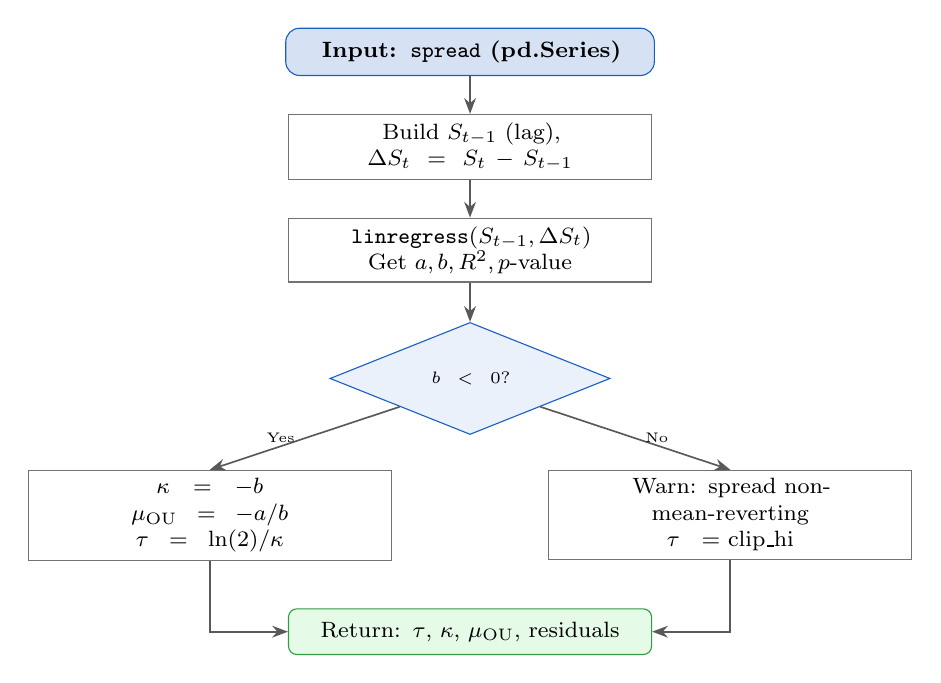
\begin{tikzpicture}[node distance=0.48cm,
                    every node/.style={font=\scriptsize}]
  \node (in) [fc_start]
    {Input: \texttt{spread} (pd.Series)};
  \node (lag) [fc_proc, below=of in]
    {Build $S_{t-1}$ (lag),\quad $\Delta S_t = S_t - S_{t-1}$};
  \node (ols) [fc_proc, below=of lag]
    {\texttt{linregress}$(S_{t-1}, \Delta S_t)$\\
     Get $a, b, R^2, p$-value};
  \node (d1) [fc_dec, below=0.5cm of ols]
    {$b < 0$?};
  \node (good) [fc_proc, below left=0.8cm and 0.1cm of d1]
    {$\kappa = -b$\\
     $\mu_{\text{OU}} = -a/b$\\
     $\tau = \ln(2)/\kappa$};
  \node (bad) [fc_proc, below right=0.8cm and 0.1cm of d1]
    {Warn: spread non-mean-reverting\\
     $\tau = $ clip\_hi};
  \node (out) [fc_out, below=2.2cm of d1]
    {Return: $\tau$, $\kappa$, $\mu_{\text{OU}}$, residuals};
  \draw[arr] (in) -- (lag);
  \draw[arr] (lag) -- (ols);
  \draw[arr] (ols) -- (d1);
  \draw[arr] (d1.south west) -- node[left,font=\tiny]{Yes} (good.north);
  \draw[arr] (d1.south east) -- node[right,font=\tiny]{No} (bad.north);
  \draw[arr] (good.south) |- (out.west);
  \draw[arr] (bad.south)  |- (out.east);
\end{tikzpicture}
}
\caption{Execution flowchart for \texttt{HalfLife.estimate()}.}
\label{fig:hl_flow}
\end{figure}

%=============================================================================
\section{Worked Example}
%=============================================================================

\begin{tcolorbox}[exbox={Setup}]
Spread: $S = [0.05, -0.10, 0.08, -0.06, 0.12, -0.03, 0.07]$.\\
We compute $S_{t-1}$ and $\Delta S_t$:
\end{tcolorbox}

\begin{center}{\small
\begin{tabular}{@{}ccc@{}}
\toprule
$t$ & $S_{t-1}$ & $\Delta S_t$\\\midrule
2 & 0.05 & $-$0.15\\
3 & $-$0.10 & 0.18\\
4 & 0.08 & $-$0.14\\
5 & $-$0.06 & 0.18\\
6 & 0.12 & $-$0.15\\
7 & $-$0.03 & 0.10\\
\bottomrule
\end{tabular}
}\end{center}

\noindent\textbf{OLS regression:}
\[
  \hat b \approx -1.60, \quad \hat a \approx -0.01
\]
\[
  \kappa = -(-1.60) = 1.60, \quad
  \tau = \frac{\ln 2}{1.60} \approx 0.43 \text{ obs}
\]

\begin{tcolorbox}[resultbox={Interpretation}]
$\tau \approx 0.43$ observations: the spread reverts in less than
1 period.  This is very fast and may indicate data noise rather than
true cointegration.  In practice, use a larger dataset.
$\hat b = -1.60 < 0$ confirms mean-reversion.
\end{tcolorbox}

%=============================================================================
\section{Python Implementation}
%=============================================================================

\begin{tcolorbox}[codebox={OU OLS Regression}]
\begin{lstlisting}[style=pythonplain]
def estimate(self) -> float:
    s = self._spread.values
    S_lag = s[:-1]      # S_{t-1}
    dS    = np.diff(s)  # delta S_t
    result = stats.linregress(S_lag, dS)
    self.b_coef = float(result.slope)
    self.a_coef = float(result.intercept)
    if self.b_coef >= 0:
        warnings.warn("b>=0: not mean-reverting")
        self.half_life_days = float(self.clip_hi)
    else:
        self.kappa  = -np.log(1.0 + self.b_coef)
        self.mu_ou  = -self.a_coef / self.b_coef
        raw_hl = np.log(2.0) / self.kappa
        self.half_life_days = float(
            np.clip(raw_hl, self.clip_lo, self.clip_hi))
    return self.half_life_days
\end{lstlisting}
\end{tcolorbox}

%=============================================================================
\section{Key Parameters Summary}
%=============================================================================

\begin{center}
{\small
\begin{tabular}{@{}p{1.5cm}p{3.2cm}p{1.0cm}@{}}
\toprule
Symbol & Meaning & Unit\\
\midrule
$\kappa$ & Mean-reversion speed & per obs\\
$\mu_{\text{OU}}$ & Long-run mean (equilibrium) & spread units\\
$\tau$ & Half-life: time for 50\% reversion & obs\\
$b$ & OLS slope; $b = -\kappa$ & —\\
$a$ & OLS intercept; $a = \kappa\mu$ & —\\
$Q$ & Kalman process noise $\approx\sigma^2_\varepsilon/\tau$ & —\\
\bottomrule
\end{tabular}
}
\end{center}

\end{document}
